%%---------------------------------------------------------------------------%%
%% draco-release.tex
%% Thomas M. Evans
%% $Id$
%%---------------------------------------------------------------------------%%
\documentclass[11pt]{nmemo}
\usepackage[centertags]{amsmath}
\usepackage{amssymb,amsthm,graphicx}
\usepackage[mathcal]{euscript}
\usepackage{tmadd,tmath}
\usepackage{cite}

%%---------------------------------------------------------------------------%%
%% DEFINE SPECIFIC ENVIRONMENTS HERE
%%---------------------------------------------------------------------------%%
%\newcommand{\elfit}{\ensuremath{\operatorname{Im}(-1/\epsilon(\vq,\omega)}}
%\msection{}-->section commands
%\tradem{}  -->add TM subscript to entry
%\ucatm{}   -->add trademark footnote about entry

\newcommand{\draco}{{\normalfont\normalsize\textsf Draco}}
\newcommand{\milagro}{{\normalfont\normalsize\textsf Milagro}}
\newcommand{\solon}{{\normalfont\normalsize\textsf Solon}}

\newcommand{\cfour}{{\normalfont\normalsize\scshape c\small 4}}
\newcommand{\dsxx}{{\normalfont\normalsize\scshape ds\raisebox{.2ex}
  {\scriptsize ++}}}

\newcommand{\stable}{{\normalfont\normalsize\texttt latest\_stable}}

%%---------------------------------------------------------------------------%%
%% BEGIN DOCUMENT
%%---------------------------------------------------------------------------%%
\begin{document}

%%---------------------------------------------------------------------------%%
%% OPTIONS FOR NOTE
%%---------------------------------------------------------------------------%%

\toms{Distribution}
%\toms{Joe Sixpak/XTM, MS B226}
\refno{XTM:TME-97-??? (U)}
\subject{Draco Release Policy and Procedures}

%-------NO CHANGES
\divisionname{Applied Theoretical \& Computational Physics Div.}
\groupname{X-TM:Transport Methods Group}
\fromms{Thomas M. Evans/XTM D409}
\phone{(505)665--3677}
\originator{tme}
\typist{tme}
\date{\today}
%-------NO CHANGES

%-------OPTIONS
%\reference{NPB Star Reimbursable Project}
%\thru{P. D. Soran, XTM, MS B226}
%\enc{list}      
%\attachments{list}
%\cy{list}
%\encas
%\attachmentas
%\attachmentsas 
%-------OPTIONS

%%---------------------------------------------------------------------------%%
%% DISTRIBUTION LIST
%%---------------------------------------------------------------------------%%

\distribution {
  XTM MS D409:\\ 
  J.E. Morel, XTM MS D409\\ 
  G.L. Olson, XTM MS D409\\ 
  J.M. McGhee, XTM MS D409\\ 
  H.G. Hughes, XTM MS D409\\ 
  T.M. Evans, XTM MS D409\\ 
  M.G. Gray, XTM MS D409\\ 
  M.L. Hall, XTM MS D409\\ 
  S. Pautz, XTM MS D409\\ 
  R.M. Roberts, XTM MS D409\\ 
  S.A. Turner, XTM MS D409\\ 
  T.J. Urbatsch, XTM MS D409\\ 
  J.S. Warsa, XTM MS D409\\
}

%%---------------------------------------------------------------------------%%
%% BEGIN NOTE
%%---------------------------------------------------------------------------%%

\opening

\section{Introduction}

The purpose of this memo is to outline the release policy and
procedures for \draco\ and \draco\ packages.  These procedures should
also apply to \draco-modeled code projects including \solon\ and
\milagro.  \draco\ products are version-controlled by {\bf cvs} tags.
Thus, releases of a particular code are simply shipped by using an
appropriate \texttt{cvs export} command.

This memo consists of two primary sections plus an Overview
(\S~\ref{sec:overview}) and Summary (\S~\ref{sec:summary}).
Section~\ref{sec:policy} outlines \draco\ release policies.  This
section contains information on the following topics:
\begin{enumerate}
\item the release policy for \draco-components;
\item the release policy for \draco;
\end{enumerate}
Section~\ref{sec:procedures} outlines the procedures for releasing
\draco\ and \draco-components.  In this section we will:
\begin{enumerate}
\item explain a general numbering scheme for \draco\ project releases;
\item show how to tag \draco\ package releases;
\item show how to tag \draco\;
\item explain how to handle bugs in a particular \draco\ release.
\end{enumerate}
Adherence to these policies will expedite code reviews in the \draco\ 
project and will present a clean interface to outside users.
Deviations from policies described herein are allowed under special
circumstances as judged by the \draco\ project team.  The \draco\ 
release procedure heavily utilizes the {\bf cvs} version control
system.  Thus, \draco\ developers should peruse the {\bf cvs}
manual~\cite{cvs} to become intimate with its controls and use.

%%---------------------------------------------------------------------------%%

\section{Overview}
\label{sec:overview}

The general release policy in \draco\ is to separate the package
release number from the \draco\ release number.  This allows \draco\ 
to have regular releases without waiting for individual packages to
get to the next release point.  For example, if the \dsxx\ package is
migrating from \texttt{ds++-1\_5\_0} to \texttt{ds++-1\_6\_0} when
\draco\ is ready for release, the \draco\ team can release a version
of \draco\ that includes \texttt{ds++-1\_5\_0}.  If \draco\ releases
are required to wait for all of its packages to move forward to the
next release point then \draco\ would never be shipped.  Separating
the \draco\ and \draco\ package release numbers eases the pressure on
\draco\ package developers who would otherwise delay \draco\ releases.

A typical release of \draco\ is illustrated in
Fig.~\ref{fig:drelease}.  Each package in \draco\ is at a closure
\begin{figure}
  \centerline{\includegraphics{drelease.eps}}
  \caption{Schematic figure of a sample \draco\ release.  Release
    number formats are explained in \S~\ref{sec:rel_num}.}
  \label{fig:drelease}
\end{figure}
point commensurate with the \draco\ release.  This entails easy access
for bug fixes for a particular version of \draco.  Release dates for
\draco\ and \draco\ packages are decided by \draco\ project
developers as explained in \S~\ref{sec:policy}.

%%---------------------------------------------------------------------------%%
 
\section{Draco Release Policies}
\label{sec:policy}

The \draco\ release policy is a set of general requirements that
control the process of software release in the \draco\ code system.
To start, we will write down the software release policies for \draco.
Afterwards, we describe these policies in more detail.  The policies
dictating \draco\ process are purposely not meticulously defined.
Because the \draco\ development team is small, only a small set of
general policies are required.  Additionally, these policies may be
waived in specific circumstances by pervue of the \draco\ development
team.

The \draco\ release policies are the following:
\begin{enumerate}
\item Each file in \draco\ will have, at a minimum, two tags, a
  \draco-level tag and a \stable\ tag.  The \stable\ tag is a
  ``pointer-like'' tag that points to the latest stable release of a
  particular \draco\ component.  The \draco\ tag is a numbered release 
  tag that refers to a fully-stable, released version of \draco.
\item Package files will have numbered release tags in addition to the 
  common tags.
\item \draco build-system components (\texttt{config/},
  \texttt{tools/}, and \texttt{templates/}) will have numbered release
  tags in addition to the common tags.
\item Additional \draco\ components such as \texttt{doc/} and
  \texttt{draco\_www} may or may not have tags in addition to the
  common tags.  This is a discretionary policy of the \draco\ team and 
  principle developers of the component.
\item \draco\ release dates are determined by the \draco development
  team.  To qualify for numbered release the following conditions must 
  be satsfied:
  \begin{itemize}
  \item All components in \draco\ must be in a tagged \stable\
    condition.
  \item All components that maintain individual numbered release tags
    should be at a numbered release.
  \item All components must pass their respective suite of
    regression tests.
  \item All \draco\ developers that have contributed to any
    components since the last release should comply with the release
    date.
  \end{itemize}
\item For a component to be placed in a \stable\ condition the
  following conditions must be satisfied:
  \begin{itemize}
  \item The component must pass its regression tests.
  \item If the component is subject to numbered release tags, it
    should receive a new numbered tag concurrent with its \stable\ 
    tag.  A \stable\ tag should always point to a numbered release
    tag, either at the package level or at the \draco\ level.
  \item All other \stable\ \draco\ components that depend upon this
    component must pass their regression tests.
  \end{itemize}
\item Major numbers on \draco\ tags should correspond to the {\bf cvs} 
  revision numbers.
\item \draco\ code packages should have a \texttt{release()} function
  that can be called from the package library.  This function returns
  a \texttt{std::string} of the numbered release tag.
\item No non-\draco\ tags should exist on \draco\ components that sit
  under the \texttt{draco/} directory in \texttt{\$CVSROOT}.
\end{enumerate}
We will now explain these policies in more detail.

\subsection{Draco Tagging Strategy}

To implement the policies layed out above, we have developed the
\stable\ tag.  Consider Fig.~\ref{fig:tag-strategy}.
 
%%---------------------------------------------------------------------------%%

\section{Draco Release Procedures}
\label{sec:procedures}

\subsection{Release Numbers}
\label{sec:rel_num}

The \draco\ project uses a uniform numbering scheme for all releases;
however, as with all components of \draco, these can be changed under
special circumstances as decided by the \draco\ development team.
\draco\ code releases are numbered according to the following scheme:
\begin{equation}
  \boldsymbol
  \langle\mathit{pkg\_name}\rangle\_
  \langle\mathit{major}\rangle.
  \langle\mathit{minor}\rangle.
  \langle\mathit{branch}\rangle\; .
  \notag
\end{equation}
In the above, $\langle\mathit{pkg\_name}\rangle$ is the name of the
package, and $\langle\mathit{major}\rangle$ and
$\langle\mathit{minor}\rangle$ are the major and minor version
numbers, respectively. Bug fixes to a particular package version are
done using {\bf cvs} branches.  A release of such a branch is noted by
$\langle\mathit{branch}\rangle$.  Release numbers are not decimal
numbers.  For example, \texttt{draco\_1.32.0} is the thirty-second
minor revision of version~1 of \draco.  Examples of some release
numbers are given below.
\begin{center}
  \begin{tabular}{ll}
    \texttt{ds++\_1.32.0} & major version~1, minor version~32 of the
    \dsxx\ package \\
    \texttt{c4\_4.12.3} & the third bug fix to major version~4, minor
    version~12 of the \cfour\ package \\
  \end{tabular}
\end{center}

Version numbers are assigned at the discretion of the package
developer.  Minor updates to a major version should be indicated by
increasing the minor version number.  Major changes or releases are
indicated by the major version number.  The package developer decides
whether a release is a major or minor revision.  The only requirement
is that the version numbers increase monotonically.  Additionally,
when updating to a new major version, the minor version number should
be reset to zero.  Thus, when moving from \texttt{c4\_1.109.0} to
version~2 of \cfour, the new version number should be
\texttt{c4\_2.0.0}.

\subsection{Tagging Draco Packages}

Version numbers of the source code are handled by {\bf cvs}.  Tagging
a \draco\ package involves two steps:
\begin{enumerate}
\item updating the version number in the \texttt{Version.cc} code
  file;
\item tagging all of the source using {\bf cvs}.
\end{enumerate}
We will quickly explain these steps.

Each \draco\ package contains the source code \texttt{Version.hh} and
\texttt{Version.cc}.  This component contains the free-function
\texttt{version()} that returns the version number of the
package\footnote{The \texttt{version()} function is wrapped in the
  package namespace to avoid global namespace contamination.}.  This
can be used in code to confirm the version number of a particular
package library.  The version number is assigned in the
\texttt{version()} function definition.  This string must be updated
when package versions are released.

The second step in releasing a \draco\ package is to tag the package
source code.  This is performed by the following {\bf cvs} command:
\begin{verbatim}
     cvs tag pkg_#.#.#
\end{verbatim}
The above command works while in the package directory.  To tag the
package at a higher directory level, simply append the package
directory name.  See the GNU {\bf cvs} manual for more information.

\subsection{Tagging Draco}

Each \draco\ release consists of a series of tagged (released)
packages.  Thus, tagging a \draco\ release involves updating each
project directory to the appropriate version and then tagging all of
\draco\ with a release tag.  For example, consider the \draco\ release 
illustrated in Fig.~\ref{fig:drelease}.  We want to make \draco\
release \texttt{draco\_1.3.0}.  This release should contain the
following packages:
\begin{verbatim}
     ds++_2.1.0
     c4_1.4.1
     xm_4.1.0
     rng_1.3.0
\end{verbatim}
Note that one bug fix has been committed to \cfour.  Since the initial
time of these package releases, a \cfour\ developer has begun working
on version~1.5 and a \dsxx\ developer has begun work on version~2.2.
Thus, the current versions of these packages in {\bf cvs} must be
reverted back to the release points. This is performed by the
following series of {\bf cvs} commands:
\begin{verbatim}
     cvs checkout draco
     cd draco/src
     cvs update -r ds++_2.1.0 ds++
     cvs update -r c4_1.4.1 c4
     cvs update -r xm_4.1.0 xm
     cvs update -r rng_1.3.0 rng
\end{verbatim}
These commands will insure that each package is in the proper state.
All that remains is to tag \draco\ itself.  This is accomplished
through {\bf cvs} using:
\begin{verbatim}
     cvs tag draco_1.3.0
\end{verbatim}
As before, this command assumes that one is in the \draco\ top-level
directory.  

On a final note, \draco-modeled systems such as \solon and \milagro\
are tagged in a similar manner.  However, the decision on whether to
tag sub-packages of these systems is left to the system developer.
For code systems that contain many sub-packages, separating package
and system level tags may be required.  For systems that contain few
source components, one tag may suffice.  The only requirement for
\draco-modeled projects is that they contain a system-level tag.
Thus, \milagro\ is required, at a minimum, to have a
\texttt{milagro\_1.0.0} tag.  Any additional tags are left to the
discretion of the project development team.

\subsection{Bug Fixes}

As alluded to in earlier sections, bugs are handled on {\bf cvs}
branches that join at a particular release.  For example, consider a
bug fix to \texttt{c4\_1.9.0} that is in \draco\ version
\texttt{draco\_1.4.0}.  A branch is generated at this release as
illustrated in Figure~\ref{fig:branch}.  To generate the branch the
\begin{figure}
  \centerline{\includegraphics[width=4in]{branch.eps}}
  \caption{Schematic of a bug-fix branch in {\bf cvs}.}
  \label{fig:branch}
\end{figure}
following {\bf cvs} commands are used:
\begin{verbatim}
     cvs checkout -r draco_1.4.0 draco
     cd draco/src/c4
     cvs tag -b c4_1.9.1
\end{verbatim}
This creates a branch to \cfour\ version~1.4.  If the bug fix is
required in a \draco\ release, \draco\ should be re-released with the
appropriate branch number.  For example, to include \texttt{c4\_1.9.1}
in a \draco\ release we tag \draco\ using:
\begin{verbatim}
     cvs checkout -r draco_1.4.0 draco
     cd draco/src
     cvs update -r c4_1.9.1 c4
     cd ..
     cvs tag draco_1.4.1
\end{verbatim}
Thus, \draco\ itself is not put on a branch.  The branch number on
\draco\ versions indicates bug fixes in \draco\ packages.

Additional fixes of bugs on package branches should be tagged using
\texttt{cvs tag c4\_1.9.2}.  Thus, to make a tag to this \cfour\ 
version use the following commands:
\begin{verbatim}
     cvs checkout -r draco_1.4.1 draco
     cd draco/src
     cvs tag c4_1.9.2 c4
     cd ..
     cvs tag draco_1.4.2
\end{verbatim}
We note that {\bf cvs} branches automatically release code to the end
of the branch.  Hence, \texttt{cvs checkout -r c4\_1.9.1 c4} will
automatically give the sources at the end of the \cfour\ branch
connected to version~1.9.  We add tags to clarify the development and
bug tracking process in \draco\ even though they may not be strictly
necessary in all cases.  For more information on branches, see
Chapter~5 of the {\bf cvs} manual.

%%---------------------------------------------------------------------------%%

\section{Summary}
\label{sec:summary}

We have explained the tagging and release procedure for \draco\ 
projects in group XTM.  As with all \draco\ procedures, exceptions to
the standard rules are acceptable pending review by \draco\ team
members.  These procedures have been reviewed and are part of the
\draco\ development process.

%%---------------------------------------------------------------------------%%

\bibliographystyle{rnote}
\bibliography{../bib/draco}

\closing
\end{document}

%%---------------------------------------------------------------------------%%
%% end of draco-release.tex
%%---------------------------------------------------------------------------%%
